\section[Closing]{Closing thoughts}
\label{sec:closing}

%---------------------------------------------------------------
% 1. Summary
%---------------------------------------------------------------
\begin{frame}{Seminar summary}

	\begin{columns}[c]
		% lessons
		\begin{column}{.45\textwidth}
		    You've learned:
		    \begin{itemize}
			    \item Why we communicate
			    \item Some ways to communicate
			    \item How to structure your communications
		    \end{itemize}
		\end{column}

		\begin{column}{.45\textwidth}
		
		    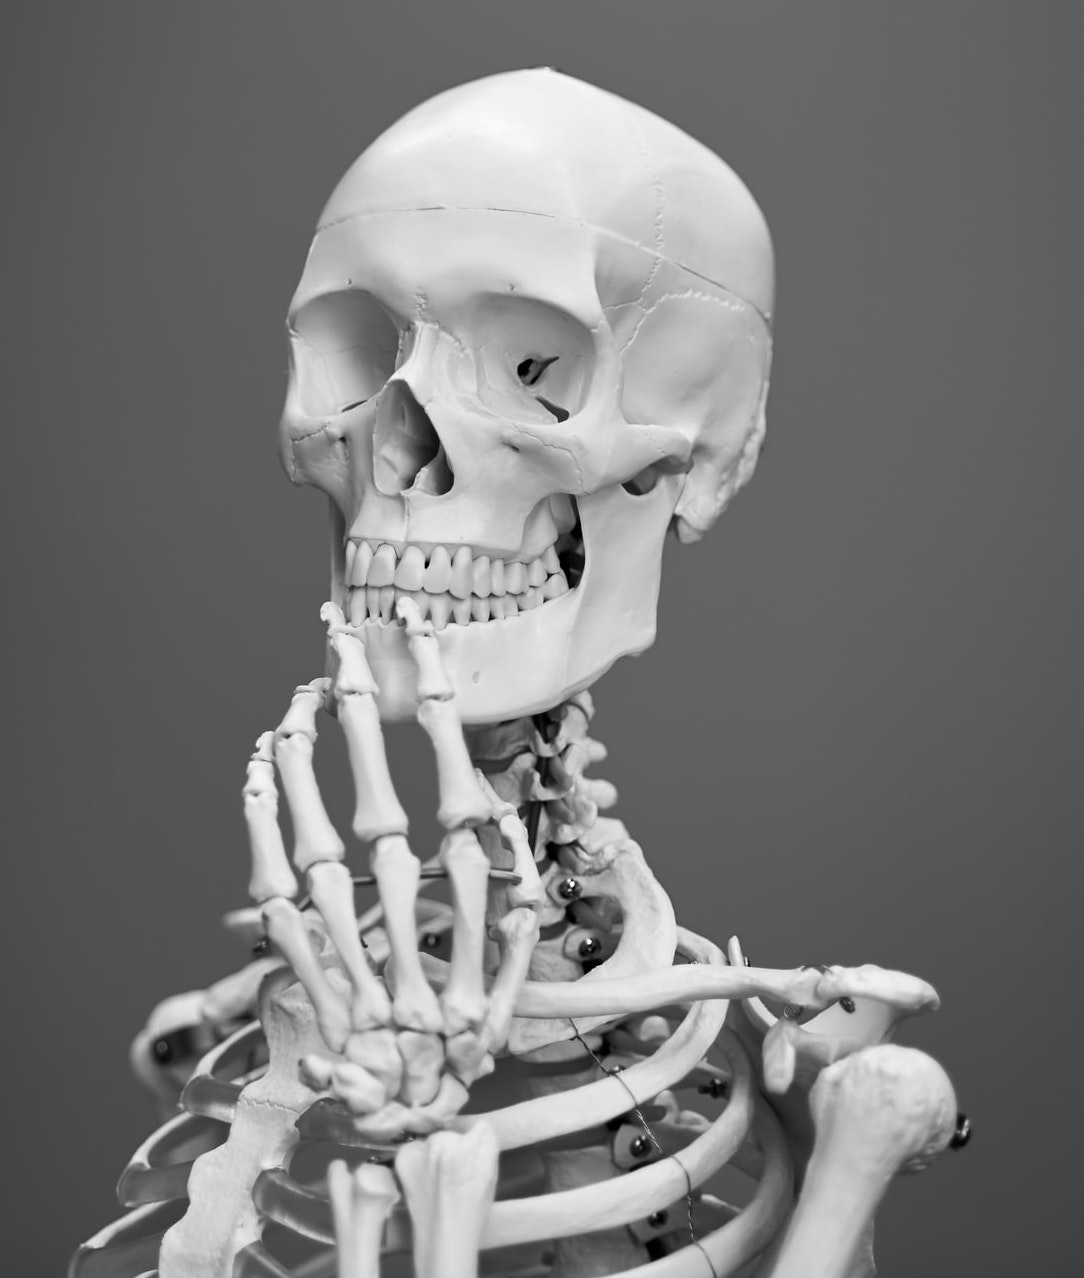
\includegraphics[width=0.85\textwidth]{images/mathew-schwartz-8rj4sz9YLCI-unsplash-crop.jpg}
		    
		    \givecredit{%
		        \centering
		        Photo by \textlink{https://unsplash.com/@cadop}{Mathew Schwartz} on \textlink{https://unsplash.com/s/photos/thinking}{Unsplash}}
		\end{column}
		
	\end{columns}

\end{frame}

%---------------------------------------------------------------
% 2. Next steps
%---------------------------------------------------------------

\begin{frame}{What to do now}

	\begin{columns}[t]
		\begin{column}{.45\textwidth}
		
		\begin{block}{Further reading}
		\begin{itemize}
		    \item \textlink{https://www.linux.com/news/birth-linux-how-linux-got-started/}{The Birth of Linux: How Linux Got Started.} (Linux.com, 2020)
		    \item \textlink{http://openbikeinitiative.org/}{The open Bike Initiative}
		\end{itemize}
		\end{block}
		
		\begin{block}{Self-study 4: Communicate!}
			Create and implement a communications strategy for two of your stakeholder groups
			\begin{itemize}
			    \item See the \textlink{https://github.com/LIKE-ITN/OpenScienceTrainingCourse/tree/master/08_selfstudy4}{guidance on GitHub}.
			\end{itemize}
		\end{block}
		\end{column}

		\begin{column}{.45\textwidth}
		
		\begin{block}{Assignment 1: Implementation Case Study}
			Prepare a case study about making your work FAIR and communicating it to your stakeholders.
			\begin{itemize}
			    \item See the \textlink{https://github.com/LIKE-ITN/OpenScienceTrainingCourse/tree/master/09_assignment1}{guidance on GitHub}.
			\end{itemize}
		\end{block}
		
		\begin{block}{Seminar 5: data management plans}
			What are data management plans, and why do they matter?
			\begin{itemize}
				\item See the \textlink{https://github.com/LIKE-ITN/OpenScienceTrainingCourse/blob/master/10_seminar5/readme.md}{Seminar materials on GitHub}
			\end{itemize}
		\end{block}
		\end{column}

	\end{columns}

\end{frame}

%---------------------------------------------------------------
% 3. Wait, what?
%---------------------------------------------------------------

\begin{frame}{A what now?}

    \textbf{Assignment 1:}\\
    Prepare a case study based on your self-study work to describe what was done to make your work FAIR and implement the R5 concepts, and how you communicated your work to your stakeholders. For example...
    \begin{itemize}
        \item Publishing your Master’s thesis through your university’s data portal and promoting it to stakeholders.
        \item Promoting results or a first paper from your LIKE PhD through websites like LinkedIn, Xing, or other social media
        \item Sharing code or other results through GitHub, Zenodo, or some other repository and sharing results with colleagues
    \end{itemize}
    
    Deliverable: Prepare a 5-minute presentation for the workshop.

\givecredit{N.B: These details may be out of date! Always check the \textlink{https://github.com/LIKE-ITN/OpenScienceTrainingCourse/blob/master/09_assignment1/readme.md}{assignment details on GitHub}.}

\end{frame}

%---------------------------------------------------------------
% 4. Let's make this open
%---------------------------------------------------------------
\begin{frame}{Let's make this presentation open}

	\begin{columns}[t]
		\begin{column}{.45\textwidth}
		  \centering
		  
\includegraphics[height=1.5cm]{images/1280px-FAIR_data_principles.jpg}

		    \givecredit{\centering Image source: \textlink{https://en.wikipedia.org/wiki/FAIR_data#/media/File:FAIR_data_principles.jpg}{Wikimedia}. Credit: \textlink{https://commons.wikimedia.org/w/index.php?title=User:SangyaPundi}{SangyaPundir}. \\
		    Reused under the \textlink{https://creativecommons.org/licenses/by-sa/4.0}{CC BY-SA 4.0 license}}
		\end{column}

		\begin{column}{.45\textwidth}
		    \centering
		    
\includegraphics[height=1.5cm]{images/cc-by-sa.png}
    \end{column}
	\end{columns}

	\begin{columns}[t]
		\begin{column}{.45\textwidth}
		    \centering
		% Findable
		    \begin{block}{Findable}
			    This presentation has a DOI: %
			    (\textlink{http://dx.doi.org/10.5281/zenodo.4034476}{10.5281/zenodo.4034476}) %
			    and has been tagged with appropriate metadata.
		    \end{block}

		    % accessible
		    \begin{block}{Accessible}
			    This presentation is archived at Zenodo.org. \\
			    The source code is available through GitHub.
		    \end{block}
    \end{column}

		\begin{column}{.45\textwidth}
		  \centering
		  \begin{block}{Interoperable}
			    This material is produced using the \LaTeX\space `Beamer' package.
		  \end{block}

		  \begin{block}{Reusable}
			  This material is reusable under the \textlink{https://creativecommons.org/licenses/by/4.0/}{CC-BY-4.0 license}.
		  \end{block}
    \end{column}
	\end{columns}
\end{frame}